\documentclass[11pt]{article}\usepackage[]{graphicx}\usepackage[]{color}
% maxwidth is the original width if it is less than linewidth
% otherwise use linewidth (to make sure the graphics do not exceed the margin)
\makeatletter
\def\maxwidth{ %
  \ifdim\Gin@nat@width>\linewidth
    \linewidth
  \else
    \Gin@nat@width
  \fi
}
\makeatother

\definecolor{fgcolor}{rgb}{0.345, 0.345, 0.345}
\newcommand{\hlnum}[1]{\textcolor[rgb]{0.686,0.059,0.569}{#1}}%
\newcommand{\hlstr}[1]{\textcolor[rgb]{0.192,0.494,0.8}{#1}}%
\newcommand{\hlcom}[1]{\textcolor[rgb]{0.678,0.584,0.686}{\textit{#1}}}%
\newcommand{\hlopt}[1]{\textcolor[rgb]{0,0,0}{#1}}%
\newcommand{\hlstd}[1]{\textcolor[rgb]{0.345,0.345,0.345}{#1}}%
\newcommand{\hlkwa}[1]{\textcolor[rgb]{0.161,0.373,0.58}{\textbf{#1}}}%
\newcommand{\hlkwb}[1]{\textcolor[rgb]{0.69,0.353,0.396}{#1}}%
\newcommand{\hlkwc}[1]{\textcolor[rgb]{0.333,0.667,0.333}{#1}}%
\newcommand{\hlkwd}[1]{\textcolor[rgb]{0.737,0.353,0.396}{\textbf{#1}}}%
\let\hlipl\hlkwb

\usepackage{framed}
\makeatletter
\newenvironment{kframe}{%
 \def\at@end@of@kframe{}%
 \ifinner\ifhmode%
  \def\at@end@of@kframe{\end{minipage}}%
  \begin{minipage}{\columnwidth}%
 \fi\fi%
 \def\FrameCommand##1{\hskip\@totalleftmargin \hskip-\fboxsep
 \colorbox{shadecolor}{##1}\hskip-\fboxsep
     % There is no \\@totalrightmargin, so:
     \hskip-\linewidth \hskip-\@totalleftmargin \hskip\columnwidth}%
 \MakeFramed {\advance\hsize-\width
   \@totalleftmargin\z@ \linewidth\hsize
   \@setminipage}}%
 {\par\unskip\endMakeFramed%
 \at@end@of@kframe}
\makeatother

\definecolor{shadecolor}{rgb}{.97, .97, .97}
\definecolor{messagecolor}{rgb}{0, 0, 0}
\definecolor{warningcolor}{rgb}{1, 0, 1}
\definecolor{errorcolor}{rgb}{1, 0, 0}
\newenvironment{knitrout}{}{} % an empty environment to be redefined in TeX

\usepackage{alltt}
\usepackage[]{style}
\usepackage[utf8]{inputenc}
\usepackage{caption}

\geometry{letterpaper, portrait, margin=1in}

\pagestyle{fancy}
\rhead{Casual \LaTeX}

\title{\vspace{2cm} \textbf{A Guide to} \LaTeX\ \textbf{ and Sweave}}
\author{}
\date{\vspace{-2cm}}


%% box S/R output
\DefineVerbatimEnvironment{Sinput}{Verbatim}{xleftmargin=2em,
                                              frame=single}
\DefineVerbatimEnvironment{Soutput}{Verbatim}{xleftmargin=2em,
                                             frame=single}
\IfFileExists{upquote.sty}{\usepackage{upquote}}{}
\begin{document}



\maketitle

\begin{center}
\Large{A casual overview}

\large Matt Lee, mlee8@g.harvard.edu, \\ Last updated: \today
\end{center}

\vspace{1em}





\tableofcontents

\pagebreak

\newgeometry{letterpaper, portrait, left=0.75in, right=1.5in, top=1in, bottom=1in,
  marginparsep = -9pt, marginparwidth = 80pt}

\section{Overview}

This document provides some basic guidelines for getting up and running with \LaTeX\ on your computer, with a specific emphasis of integrating with \texttt{R} Sweave. It is by no means all-inclusive, and the world of typesetting is quite large. Here, we'll illustrate some of the most common scenarios you might encounter when using \LaTeX\ for your reports, presentations, etc. For another great overview, check out \href{https://www.overleaf.com/learn/latex/Learn_LaTeX_in_30_minutes}{this guide by Overleaf.}

\textbf{A note}: There is a whole related world of using markdown and/or \texttt{R} markdown syntax to typeset your documents. That material will not be presented here, since its use is excellently detailed by Yihui Xie.\footnote{https://bookdown.org/yihui/rmarkdown/} 

\textbf{A disclaimer}: Proficiency in \LaTeX\ is a lifelong journey, and this document should certainly not be used as a definitive guide to best practices. This is just a semi-structured write up of how \textbf{I} use Sweave and \LaTeX\ in my own workflow, and should probably be read with a grain of salt. 

The raw files for this guide are located at \href{https://github.com/leem26/latex-intro}{this GitHub repository}. I've also included the actual homework template I use for my classes, so feel free to use that as a starting place if desired. 

\subsection{What is \LaTeX?}

\LaTeX (pronounced \textit{LAH-} or \textit{LAY-tek}) is a syntax language that is used to typeset documents. It's great for creating reports and presentations that look professional (even ``pretty''!), and is particularly useful when typesetting mathematical expressions. \LaTeX\ is also great for reproducibility, since there is a ``script'' file that documents how the output file (generally a .pdf) was created and styled. 

\subsection{What is \texttt{R} Sweave?}

Sweave is a system that allows us to integrate \texttt{R} code and output with \LaTeX\ typesetting. This has been particularly helpful for me for all of my homework assignments and working analysis documents, since I don't need to worry about remembering whether I've copied and pasted the most updated results into a word document. All I need to do is update my code (which is written directly into the Sweave .Rnw file) and re-compile it into my final PDF. 

\subsection{Reasons to use/not use \LaTeX\ }

\begin{itemize}
  \item \textbf{pro: }\LaTeX\ and Sweave are flexible, incredibly powerful, and provide a certain aesthetic that may be appealing depending on your own preferences. 
  \item \textbf{pro: }\LaTeX\ is the preferred method of typesetting used in any math-related field (e.g. biostatistics), so if you will be working in a related space it's probably worth it to learn.
  \item \textbf{con: }\LaTeX\ can have a steep learning curve and sometimes takes longer relative to other word-processing software like Microsoft Word. 
\end{itemize}

\marginnote{\textit{In practice, my general workflow is to have a set template and style I can re-use for all of my homework assignments. This saves some time and prevents me from having to start from scratch every time. But YMMV and whatever works for you, works.}}[-7cm]

\pagebreak
\section{Getting started}


\subsection{Install \TeX\ }

\TeX\ is the programming foundation of \LaTeX. You will probably never have to interact with it directly. All of the commands and text you write in your .tex or .Rnw files get interpreted by \TeX, which handles the production of the final document. 

There are many distributions of \TeX\ available, and you will need to download a version that works with your operating system (e.g. MacTeX for Mac OS and MiKTeX for Windows). You can look at the different options \href{https://www.latex-project.org/get/}{here} and follow the specific directions for each. This is generally the most comprehensive way of installing \TeX, and as a results can take quite a long time to download (e.g., MacTeX is roughly 4 Gb). 

There is a separate option tailored for \texttt{R} users called \href{https://yihui.org/tinytex/}{TinyTeX} that doesn't include every \LaTeX\ package, but is significantly smaller in file size (150 Mb on Mac OS or 220 Mb on Windows). This might be useful if you only occasionally use \LaTeX\ or don't have a ton of storage space on your computer. 


\subsection{Install \texttt{knitr} and create a new Sweave file in RStudio}

\texttt{knitr}\footnote{https://yihui.org/knitr/} is an \texttt{R} package that can be used to ``weave'' or compile your Sweave .Rnw files. To install:

\begin{enumerate}
\item Open RStudio, and type \texttt{install.packages('knitr')} into the console window. 
  \begin{figure}[H]
    \centering 
    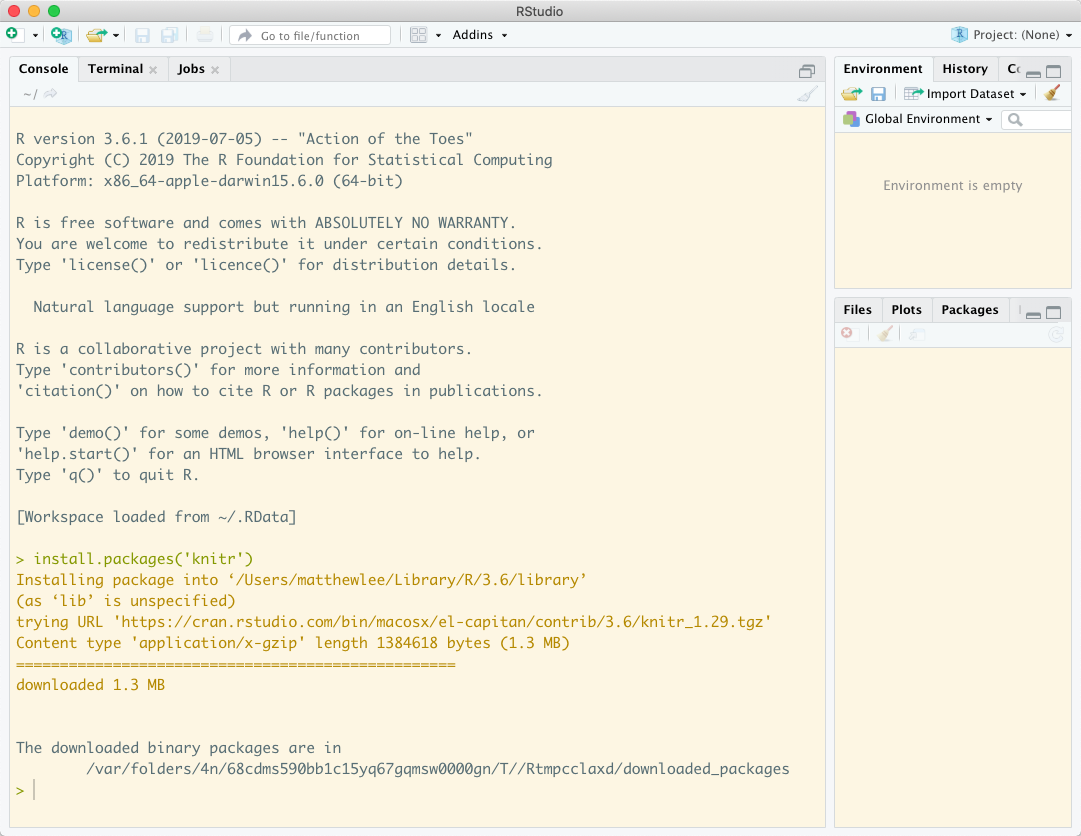
\includegraphics[width = 0.85\textwidth]{img/installknitr}
  \end{figure}
\item Create your first Sweave document! In RStudio, go to File $\rightarrow$ New File $\rightarrow$ R Sweave
  \begin{figure}[H]
    \centering
    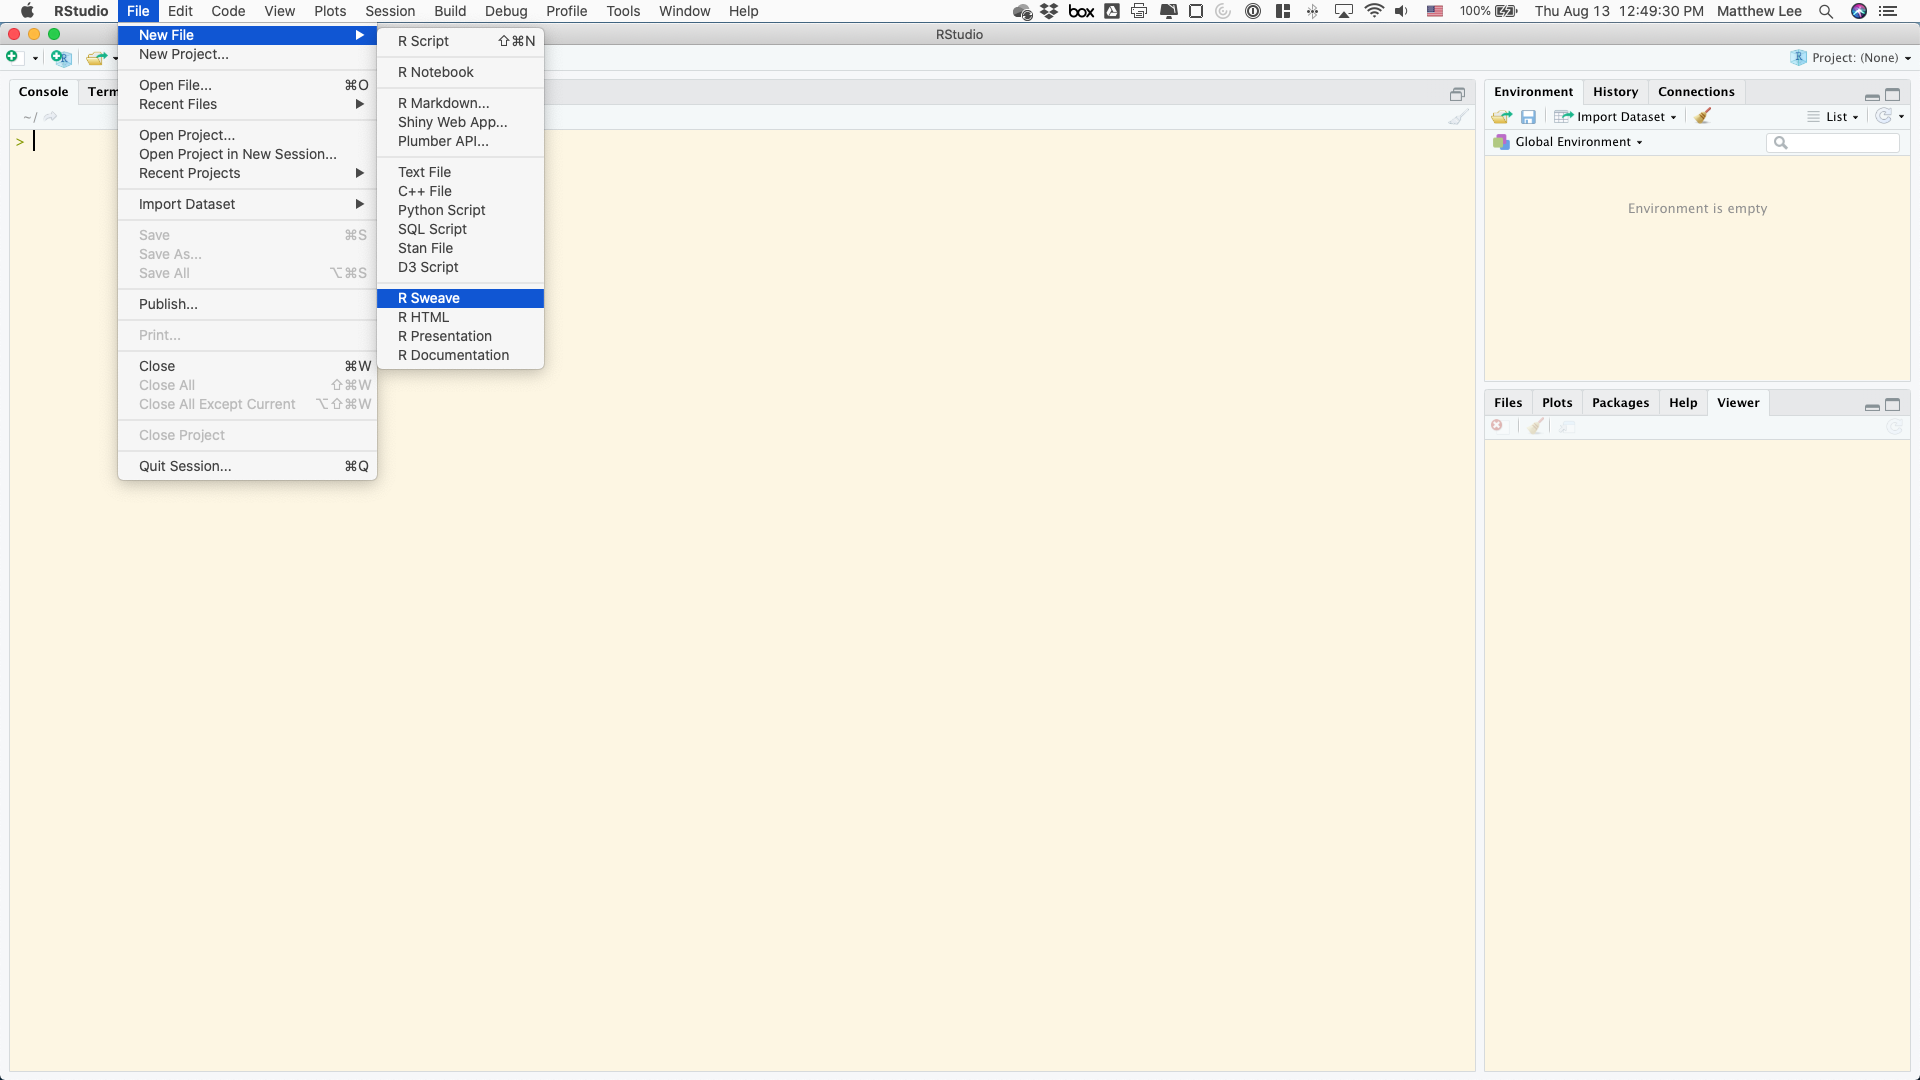
\includegraphics[width = 0.9 \textwidth]{img/newsweave}
  \end{figure}
\item Save your Sweave file, using command/ctrl + s or  File $\rightarrow$ Save. You'll notice that when you go to this file in your directory, it has the extension .Rnw. This is the extension for all Sweave files. (.Rmd is for R markdown, .R is for pure R scripts). 
\item Your Sweave file should look fairly empty, type in a message in between the \Verb#\begin{document}# and \Verb#\end{document}# tags, like below. Delete the \Verb#\SweaveOpts{concordance=TRUE}# line (this is only used when we knit using Sweave. In this case, we will knit using \texttt{knitr}). To tell RStudio that we would like to knit using \texttt{knitr}, we also need to include the line \verb# % !Rnw weave = knitr# at the very beginning. Our file should look like:

\begin{Verbatim}[frame=single]
% !Rnw weave = knitr
\documentclass{article}

\begin{document}

Hello this is a new sweave document!

\end{document}
\end{Verbatim}
\item Click ``Compile PDF'' or hit command/ctrl + shift + k on your keyboard to compile your document and output it into a PDF file. You should get a pop-up that looks something like:

  \begin{figure}[H]
    \centering 
    
\includegraphics[width = 0.8\textwidth]{img/testpdf}
  \end{figure}

\end{enumerate}

Doesn't look that great, but we will follow this basic procedure as we add to our Sweave file! You can also access some preferences for Sweave documents, like whether to preview the document after each compile, the default weave system (Sweave or knitr), and the default \LaTeX program to use to generate the PDF file, by going to Rstudio $\rightarrow$ Preferences $\rightarrow$ Sweave.

\pagebreak
\section{Structuring a Sweave/\LaTeX\ File}

\DefineShortVerb{\|}
\SaveVerb{Verb1}|\documentclass{}|
\SaveVerb{Verb2}|...|
\SaveVerb{Verb3}|\begin{document}|
\SaveVerb{Verb4}|\end{document}|


\marginnote{\textit{The general structure of a \LaTeX\ file:}   \UseVerb{Verb1} \UseVerb{Verb2} \UseVerb{Verb3} \UseVerb{Verb2} \UseVerb{Verb4}}[0cm] Every Sweave file is basically a \LaTeX\ file with the added functionality of including \verb#R# commands. As such, we need to follow \LaTeX\ rules for structuring our document. Every Sweave file should have:

\begin{itemize}
\item A \textit{Preamble}
\item A \textit{Document} environment
\end{itemize}

To comment out text, include the ``\%'' symbol at the front of the comment. 

\subsection{The Preamble}

The \textit{preamble} portion of a document is where we declare the \textbf{document class} as well as any global packages, functions, or options we want to use for our document. Let's take a look at an example that builds off of new Sweave file we created in the previous section:

\begin{Verbatim}[frame=single]
% !Rnw weave = knitr
\documentclass{article}
\usepackage[]{/Users/matthewlee/style}
\usepackage[utf8]{inputenc}
\usepackage{caption}
\usepackage{geometry}

\geometry{letterpaper, portrait, margin=1in}

\pagestyle{fancy}
\rhead{A guide to \LaTeX}

\title{\vspace{2cm} \textbf{A Guide to} \LaTeX\ \textbf{ and Sweave}}

\begin{document}

\maketitle

Hello this is a new sweave document!


\end{document}
\end{Verbatim}

\pagebreak
\marginnote{\textit{You can specify options before or after the argument, but I like to include them before for consistency.}}[1cm] We see that there's a whole bunch of lines that start with a backslash ``\textbackslash'' and end with some text enclosed in curly braces ``\{\}''. These are \textbf{functions (also called macros or commands)} in \LaTeX, where the function \textit{name} immediately follows the backslash, and function \textit{arguments} are enclosed in the brackets. \textbf{Options} for functions are enclosed by square brackets ``[]'', and can be omitted if you don't have any options to declare. 

Functions come from the \LaTeX packages you've installed on your computer with your specific distribution (e.g. MacTeX, MiKTeX, TinyTeX), or can be defined manually using the \verb#\newcommand{}# function. 

The preamble of our Sweave file is anything that comes before the \verb$\begin{document}$ command. In the example above, our preamble is:

\begin{Verbatim}[frame=single]
% !Rnw weave = knitr
\documentclass{article}
\usepackage[]{/Users/matthewlee/style}
\usepackage[utf8]{inputenc}
\usepackage{caption}
\usepackage{geometry}

\geometry{letterpaper, portrait, margin=1in}

\pagestyle{fancy}
\rhead{A guide to \LaTeX}

\title{\vspace{2cm} \textbf{A Guide to} \LaTeX\ \textbf{ and Sweave}}
\end{Verbatim}

The \textbf{document class} function at the very top, \verb#\documentclass{}# tells \TeX\ what standard layout to use for the output. There are a variety of arguments available, but the most common are ``article'', ``report'', ``book'', or ``beamer'' (for presentations). For homework assignments, I generally use the ``article'' document class and customize using different packages and options. \verb#\documentclass{}# has several options including font size, paper size and columns. For example, the command below:

\begin{center}
\begin{BVerbatim}
\documentclass[11pt, letterpaper, twocolumn]{article}
\end{BVerbatim}
\end{center}

Sets the font size to 11pt, the output to letter paper size (8.5in x 11in), and splits the document into two columns. Another way to do this is with the \texttt{geometry} package's \verb#\geometry{}# command. In the example above, I've set my formatting to letter paper, portrait orientation, and 1-inch margins with the following line:

\begin{center}
\begin{BVerbatim}
\geometry{letterpaper, portrait, margin=1in}
\end{BVerbatim}
\end{center}

In order to use this command, however, I need to tell \TeX\ to load the package that it belongs to. This is another component of the \textbf{preamble}. Before I call \verb#\geometry{}#, I use the \verb#\usepackage{}# command to to load the \texttt{geometry} package:

\begin{center}
\begin{BVerbatim}
\usepackage{geometry}
\end{BVerbatim}
\end{center}

\subsubsection{Style files}

If there are many packages you need to load, it is sometimes convenient to include them in a separate ``style'' file. This is a text file with the extension \textbf{.sty} that we call in our main document in order to load all the packages contained in our style file. In our example, I actually do this using the command:

\begin{center}
\begin{BVerbatim}
\usepackage[]{/Users/matthewlee/style}
\end{BVerbatim}
\end{center}

An excerpt from the actual style file, ``style.sty'' looks like:
\marginnote{\textit{I save my full style.sty file (which contains packages and settings relevant to creating articles and reports) in my home directory and reference it most times I write up an assignment. In cases where I need something specific, I'll create a custom style.sty file and place it in the same folder that my .Rnw file is located}}[-3cm]

\begin{Verbatim}[frame=single]
%%%%%%%%%%%%%%%%%%%%%%%%%%%%%%%%%%%%%%%%%%%%%%%%%%%%%%%%%%%%%%
%%
%% TEXT/PAGE FORMATTING PACKAGES
%%
%%%%%%%%%%%%%%%%%%%%%%%%%%%%%%%%%%%%%%%%%%%%%%%%%%%%%%%%%%%%%%

\usepackage{enumitem}
\usepackage{fancyhdr}
  \setlength{\headheight}{12pt}
\usepackage{float}
\usepackage{parskip}
  \parskip=8pt %% set parskip to 8pt
\usepackage[bottom]{footmisc}
\usepackage{changepage}
\usepackage{rotating}
\usepackage{fancyvrb}
\usepackage{lscape}
  \allowdisplaybreaks
\usepackage{marginnote}

%%%%%%%%%%%%%%%%%%%%%%%%%%%%%%%%%%%%%%%%%%%%%%%%%%%%%%%%%%%%%%
%%
%% FIGURES
%%
%%%%%%%%%%%%%%%%%%%%%%%%%%%%%%%%%%%%%%%%%%%%%%%%%%%%%%%%%%%%%%
\usepackage{graphicx}
\usepackage{subcaption}
\usepackage{wrapfig}

%%%%%%%%%%%%%%%%%%%%%%%%%%%%%%%%%%%%%%%%%%%%%%%%%%%%%%%%%%%%%%
%%
%% TABLES
%%
%%%%%%%%%%%%%%%%%%%%%%%%%%%%%%%%%%%%%%%%%%%%%%%%%%%%%%%%%%%%%%

\usepackage{cellspace, boldline}
  \setlength\cellspacetoplimit{5pt}
  \setlength\cellspacebottomlimit{2pt}
\usepackage{threeparttable, tablefootnote}
\usepackage{booktabs}
\usepackage[table,xcdraw,dvipsnames]{xcolor}
\usepackage{longtable}
\usepackage[export]{adjustbox}
\usepackage{multicol}
\usepackage{multirow}
\usepackage{makecell} 
\usepackage{tabularx}

%% Define column with grey background fill
\definecolor{Gray}{gray}{0.85}
\newcolumntype{a}{>{\columncolor{Gray}}C}
\end{Verbatim}

This just saves some space and makes reading the Sweave files a bit easier. However, you do have to be careful about package \textbf{conflicts}, which can occur if you load two packages that aren't compatible with each other. When you try to knit your file in these cases, you'll get an error. I've found that this is most common with packages related to references and bibliography settings.


\subsubsection{Other things I often do in the preamble}

In our example preamble, there are few other commands I use that help set up the layout of the document. 

\begin{itemize}
\item \verb#\pagestyle{fancy}#: Sets the page style to ``fancy'' (draws horizontal line separating the header from the main text, and lists the current section on the left side of the header) from the \texttt{fancyhdr} package.
\item \verb#\rhead{A guide to \LaTeX}#: Specifies that the right side header should include the text: ``A guide to \LaTeX''
\item \verb#\title{\vspace{2cm} \textbf{A Guide to} \LaTeX\ \textbf{ and Sweave}}#: Sets the title to \textbf{A Guide to} \LaTeX\ \textbf{ and Sweave}
\end{itemize}

\subsection{The Document Environment}

The document environment consists of all the text in between \verb#\begin{document}# and \verb#\end{document}#, and contains all of the actual content that you want to print to the output PDF file. In our example, the document environment consists of a title and a single line of content:


\begin{Verbatim}[frame=single]
\begin{document}

\maketitle 

Hello this is a new sweave document!

\end{document}
\end{Verbatim}

Note that the \verb#\maketitle# command can also print out values for ``author'' and ``date'' if you define them in your preamble (i.e. using \verb#\author{}# and \verb#\date{}#). Let's look at what our example looks like as a PDF. I've included some random example text and math just to illustrate how things appear for multiple pages:

\begin{figure}[H]
    \centering 
    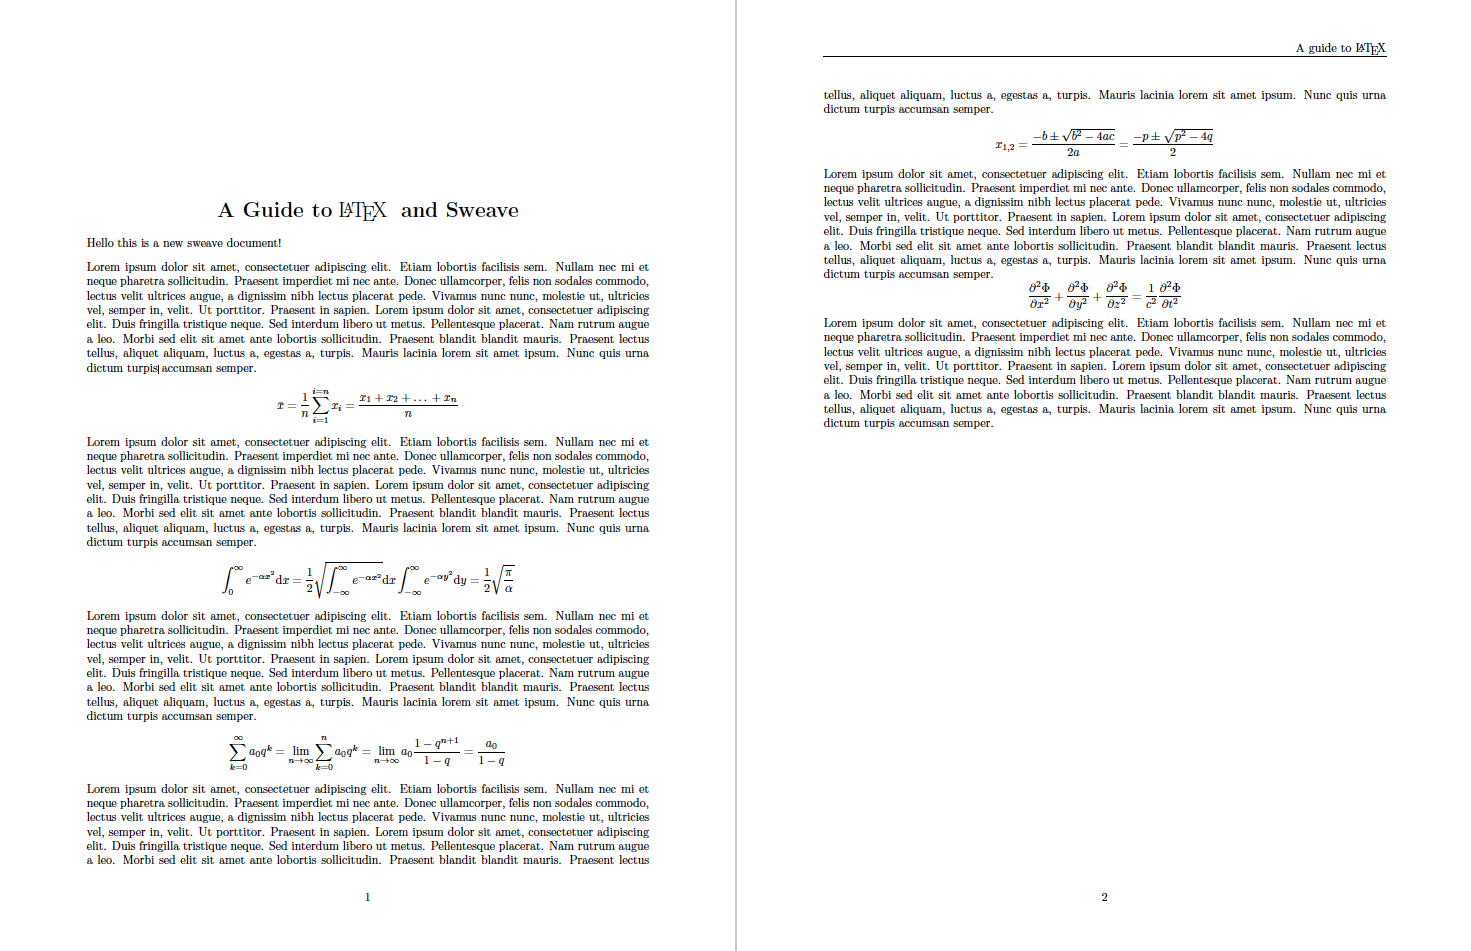
\includegraphics[width = \textwidth]{img/test2page}
\end{figure}

\section{Including R code in your Sweave file}

To include \texttt{R} code in your document, we need to tell Sweave how to recognize code vs. actual text. For Sweave, this is given by the syntax:


\verb#            <<>>=#

\begin{BVerbatim}[frame=single]
            # Here is some R code

            x <- rnorm(n = 100, mean = 25, sd = 3)
            hist(x)
\end{BVerbatim}

\verb#            @#

Where we enclose all of our \texttt{R} code inside the ``\texttt{<<>>=}'' and ``\texttt{@}'' symbols. In RStudio, the shortcut to insert these symbols automatically is \textbf{command/control + alt + i}. The code chunk above, when evaluated, looks like:

\begin{knitrout}\small
\definecolor{shadecolor}{rgb}{0.969, 0.969, 0.969}\color{fgcolor}\begin{kframe}
\begin{alltt}
\hlstd{x} \hlkwb{<-} \hlkwd{rnorm}\hlstd{(}\hlkwc{n} \hlstd{=} \hlnum{100}\hlstd{,} \hlkwc{mean} \hlstd{=} \hlnum{25}\hlstd{,} \hlkwc{sd} \hlstd{=} \hlnum{3}\hlstd{)}
\hlkwd{hist}\hlstd{(x,} \hlkwc{breaks} \hlstd{=} \hlnum{20}\hlstd{)}
\end{alltt}
\end{kframe}
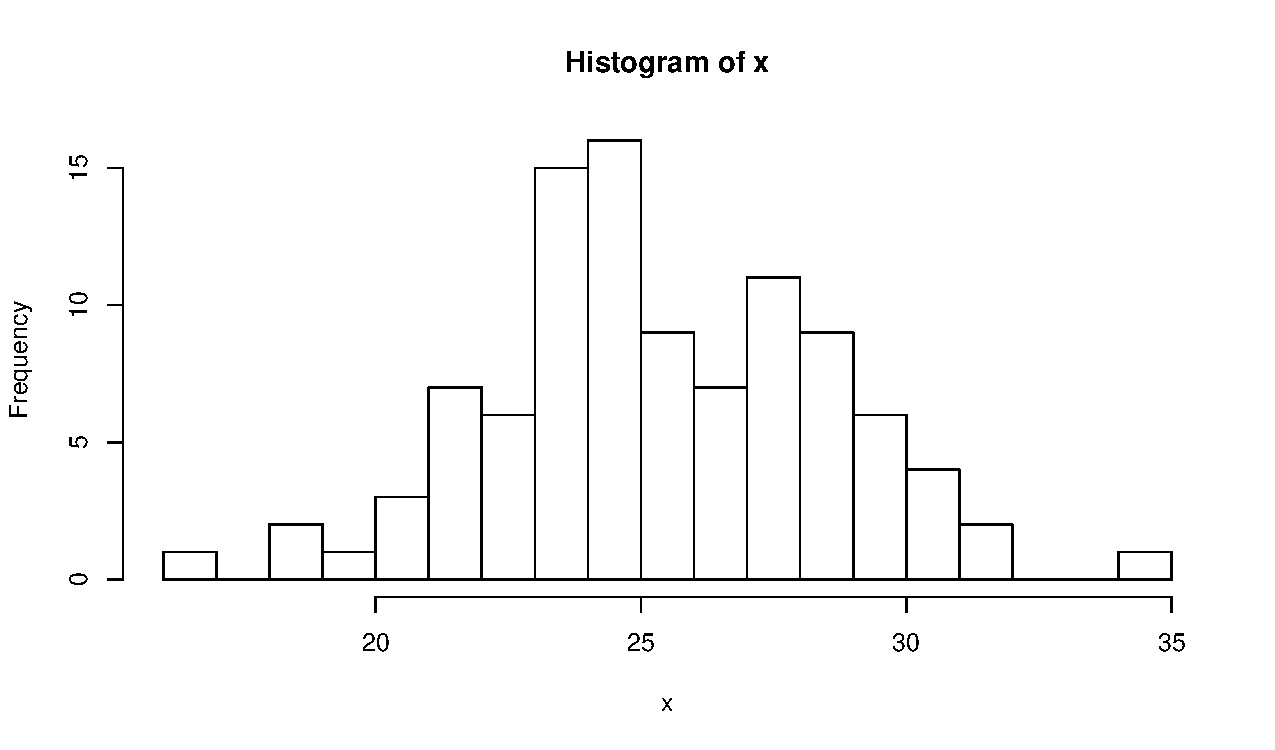
\includegraphics[width=\maxwidth]{figure/unnamed-chunk-2-1} 

\end{knitrout}

We can also specify options for our code output by specifying them in between the double left and right inequality signs. For example: 

\verb#            <<size='small', fig.height=3, fig.width=8.5, echo=TRUE, cache=TRUE>>=#

\begin{BVerbatim}[frame=single]
            # Here is some R code

            x <- rnorm(n = 100, mean = 25, sd = 3)
            hist(x)
\end{BVerbatim}

\verb#            @#


Specifies that we want our code font size to be ``small'', figure heights to be 3 inches, figure widths to be 8.5 inches, our code to be ``echo''d (i.e. repeated back to us rather than hidden), and our objects to be cached. With these new options, our code chunk looks like:

\begin{knitrout}\small
\definecolor{shadecolor}{rgb}{0.969, 0.969, 0.969}\color{fgcolor}\begin{kframe}
\begin{alltt}
\hlstd{x} \hlkwb{<-} \hlkwd{rnorm}\hlstd{(}\hlkwc{n} \hlstd{=} \hlnum{100}\hlstd{,} \hlkwc{mean} \hlstd{=} \hlnum{25}\hlstd{,} \hlkwc{sd} \hlstd{=} \hlnum{3}\hlstd{)}
\hlkwd{hist}\hlstd{(x,} \hlkwc{breaks} \hlstd{=} \hlnum{20}\hlstd{)}
\end{alltt}
\end{kframe}
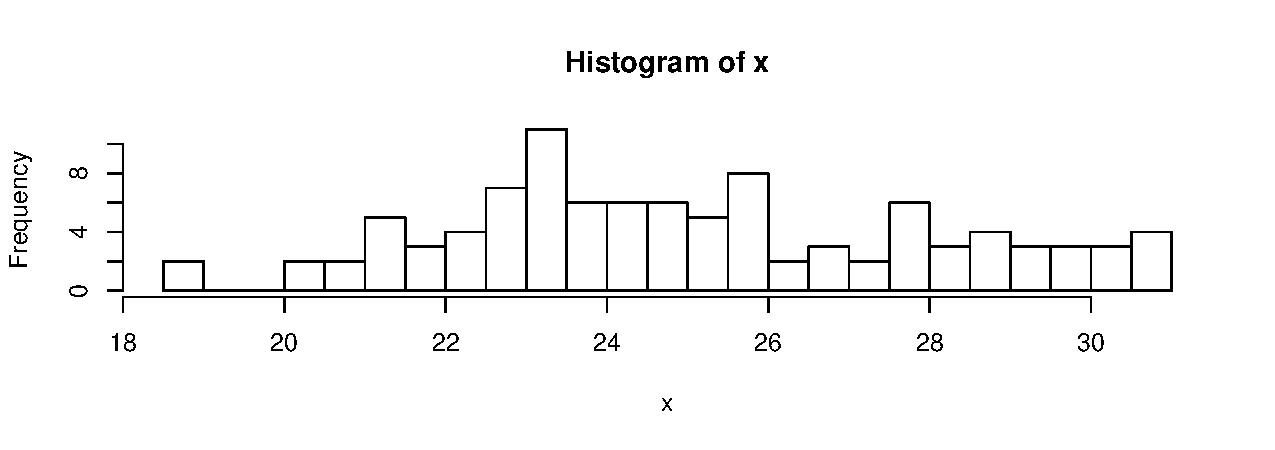
\includegraphics[width=\maxwidth]{figure/unnamed-chunk-3-1} 

\end{knitrout}

\marginnote{\textit{Why \texttt{Sexpr}? Because the \texttt{S} programming language was the precursor to what we now know as \texttt{R}. \texttt{Sexpr} stands for ``\texttt{S} expression''}}
If we want to include \texttt{R} output within a line, for example as part of a results paragraph, we can use the command \verb#\Sexpr{}# where we place whatever \texttt{R} command we want to include inside the curly braces. Let's say we want to report the mean value of x, rounded to two decimal places. We would have:

\begin{center}
The mean of x is \verb#\Sexpr#\texttt{\{round(mean(x),2)\}}
\end{center}

Show up as:

\begin{center}
The mean of x is 25.09
\end{center}

We can also use additional \texttt{R} packages with Sweave, just like with R Markdown:

\begin{knitrout}\small
\definecolor{shadecolor}{rgb}{0.969, 0.969, 0.969}\color{fgcolor}\begin{kframe}
\begin{alltt}
\hlkwd{library}\hlstd{(ggplot2)}
\hlstd{x} \hlkwb{<-} \hlkwd{as.data.frame}\hlstd{(x)}
\hlkwd{ggplot}\hlstd{(x)} \hlopt{+}
  \hlkwd{geom_bar}\hlstd{(}\hlkwd{aes}\hlstd{(}\hlkwc{x} \hlstd{= x),} \hlkwc{stat} \hlstd{=} \hlstr{"density"}\hlstd{)} \hlopt{+}
  \hlkwd{theme_bw}\hlstd{()}
\end{alltt}
\end{kframe}
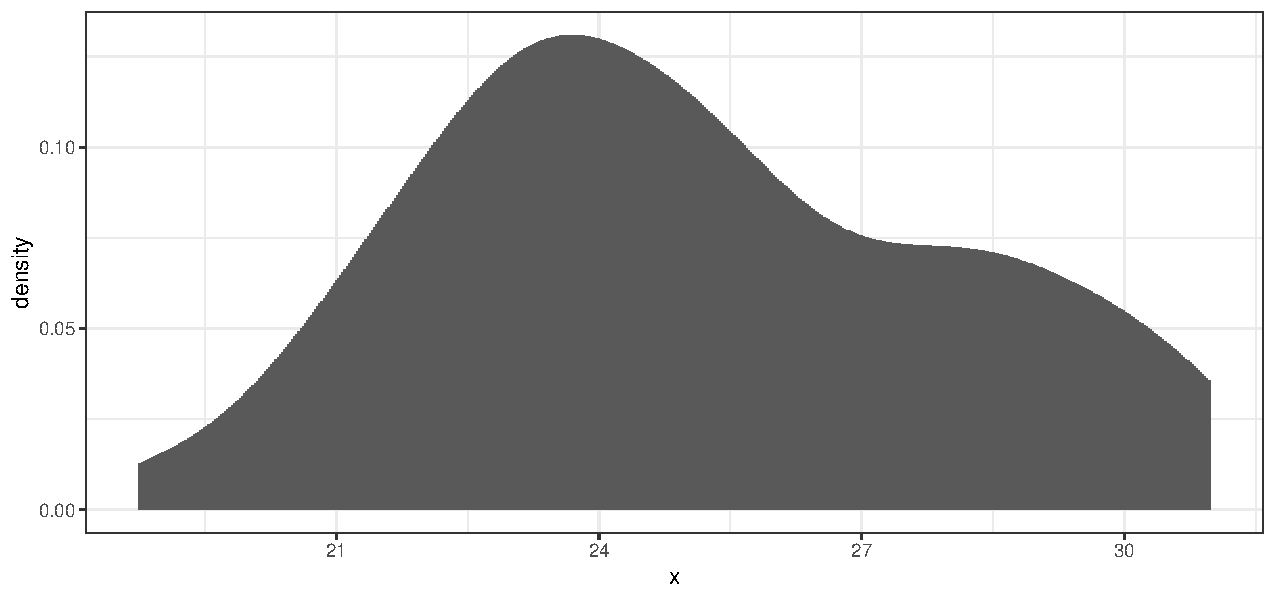
\includegraphics[width=\maxwidth]{figure/unnamed-chunk-4-1} 

\end{knitrout}


\section{Typesetting math expressions}

If you're typesetting anything with math, it's usually prudent to load the following packages either in your preamble or a separate style file:

\begin{itemize}
\item \verb#\usepackage{amsmath}#
\item \verb#\usepackage{mathtools}#
\item \verb#\usepackage{amsfonts}#
\item \verb#\usepackage{hyperref}#
\end{itemize}

\subsection{Inline mode} 

There are a number of ways to include math expressions in Sweave/\LaTeX. To include an expression ``inline'', i.e. in the line that you are writing in, surround the expression in single dollar signs (\$...\$). 

For example, ``\verb#$E(Y \mid X) = \beta_0 + \beta_1 X$# is a regression model'' will be typeset as ``$E(Y \mid X) = \beta_0 + \beta_1 X$ is a regression model''

\subsection{Display mode}

To typeset expressions in ``display mode'', i.e. expressions on separate lines, our options become a bit more diverse. The most common options are:


For quick, centered, single expressions: enclose the expression in double dollar signs or backslash-brackets (i.e. \$\$...\$\$ or \verb#\[...\]#)\footnote{https://tex.stackexchange.com/questions/503/why-is-preferable-to}. \marginnote{\textit{I've never really noticed a big difference between using double-dollar signs or backlash-brackets, but people online seem to prefer the latter due to spacing issues.}}[-0.5cm]

For example: 

\begin{center}
\begin{Verbatim}[frame=single]
$$E(Y \mid X) = \beta_0 + \beta_1 X$$

\[E(Y \mid X) = \beta_0 + \beta_1 X\]
\end{Verbatim}
\end{center}

will render as:

$$E(Y \mid X) = \beta_0 + \beta_1 X$$
\[E(Y \mid X) = \beta_0 + \beta_1 X\]


For equations that are long and need to be split into multiple lines, or multiple equations that need to be aligned, we can use environments from the \verb#amsmath# package. 

\begin{itemize}
\item If you want to write a single equation on a single line, you can use the options from above \textbf{or} use the \texttt{equation} environment if you want to ``tag'' the equation with a number. When you tag equations, \LaTeX\ will keep track of them for you and allow you to reference them if you specify a label using the \verb#\label{}# command. 

For example: 

\begin{Verbatim}[frame=single]
\begin{equation}
\label{myequation}
E(Y \mid X) = \beta_0 + \beta_1 X
\end{equation} 
\end{Verbatim}

Will get rendered as:

\begin{equation}
\label{myequation}
E(Y \mid X) = \beta_0 + \beta_1 X
\end{equation} 

And we can reference this automatically, i.e. \verb#\autoref{myequation}# (from the \texttt{hyperref} package) appears as \autoref{myequation}.

\item If we have a single expression that needs to be split across multiple lines, we can use the \texttt{split} environment \textbf{inside} the \texttt{equation} environment. To separate lines, use a double backslash ``\verb#\\#'' at the end of each line. To align lines, include an ampersand right before the position you want to align by. For example, the command below will align the two lines by the ``='' signs. 

\begin{Verbatim}[frame=single]
\begin{equation}
\begin{split}
\label{myequation2}
E(Y \mid X) &= \beta_0 + \beta_1 X \\
E(Y \mid W) &= \alpha_0 + \alpha_1 W
\end{split}
\end{equation} 
\end{Verbatim}

Will be rendered as:

\begin{equation}
\begin{split}
\label{myequation2}
E(Y \mid X) &= \beta_0 + \beta_1 X \\
E(Y \mid W) &= \alpha_0 + \alpha_1 W
\end{split}
\end{equation} 

\item If we have a long expression that needs to be split across multiple lines, but we don't care about aligning them, we can use the \texttt{multline} environment, which will align the first line to the left and the second to the right. Again, use a double backslash to separate lines. For example:

\begin{Verbatim}[frame=single]
\begin{multline}
E(Y \mid X, W, L) = \beta_0 + \beta_1 X_1 + \beta_2 X_2 + \beta_3 X_3 \\
+ \alpha_0 + \alpha_1 W_1 + \alpha_2 W_2 + \alpha_3 W_3 + \alpha_4 W_4
+ \delta_0 + \delta_1 L_1 + \delta_2 L_2 + \delta_3 L_3 + \delta_4 L_4
\end{multline}
\end{Verbatim}

Will be rendered as: 
\begin{multline}
E(Y \mid X, W, L) = \beta_0 + \beta_1 X_1 + \beta_2 X_2 + \beta_3 X_3 \\
+ \alpha_0 + \alpha_1 W_1 + \alpha_2 W_2 + \alpha_3 W_3 + \alpha_4 W_4
+ \delta_0 + \delta_1 L_1 + \delta_2 L_2 + \delta_3 L_3 + \delta_4 L_4
\end{multline}

\item If we have multiple equations (and we want to tag both separately), we can use the \verb#align# environment. Again, separate lines with double backslashes and align using ampersands:

\begin{Verbatim}[frame=single]
\begin{align}
E(Y \mid X) &= \beta_0 + \beta_1 X \\
E(Y \mid W) &= \alpha_0 + \alpha_1 W
\end{align} 
\end{Verbatim}

\begin{align}
E(Y \mid X) &= \beta_0 + \beta_1 X \\
E(Y \mid W) &= \alpha_0 + \alpha_1 W
\end{align}


\item If we want to have multiple equations, but don't care about alignment, we can use the \verb#gather# environment:

\begin{Verbatim}[frame=single]
\begin{gather}
E(Y \mid X) = \beta_0 + \beta_1 X_1 + \beta_2 X_2 \\
E(Y \mid W) = \alpha_0 + \alpha_1 W
\end{gather} 
\end{Verbatim}

\begin{gather}
E(Y \mid X) = \beta_0 + \beta_1 X_1 + \beta_2 X_2 \\
E(Y \mid W) = \alpha_0 + \alpha_1 W
\end{gather} 

\end{itemize}


For any environment where we don't want to tag the equation, we can add the ``*'' symbol to the command name. For example:

\begin{Verbatim}[frame=single]
\begin{gather*}
E(Y \mid X) = \beta_0 + \beta_1 X_1 + \beta_2 X_2 \\
E(Y \mid W) = \alpha_0 + \alpha_1 W
\end{gather*} 
\end{Verbatim}

\begin{gather*}
E(Y \mid X) = \beta_0 + \beta_1 X_1 + \beta_2 X_2 \\
E(Y \mid W) = \alpha_0 + \alpha_1 W
\end{gather*} 


\subsection{Common math expressions for PHS 2000 and beyond}


\subsubsection{For regression equations}

\textbf{Greek letters}: 

\begin{Verbatim}[frame=single]
\[
\alpha , \beta , \delta ,  \varepsilon , \gamma , \psi , \Psi, \Sigma , \gamma 
\]
\end{Verbatim}

\[
\alpha , \beta , \delta , \varepsilon ,  \gamma , \psi , \Psi, \Sigma , \gamma 
\]

To get bold math symbols, use the \verb#\bm{}# command from the \verb#bm# package:

\begin{Verbatim}[frame=single]
\[
\bm{\alpha} , \bm{\beta} , \bm{\delta} ,  \bm{\varepsilon}
\]
\end{Verbatim}

\[
\bm{\alpha} , \bm{\beta} , \bm{\delta} ,  \bm{\varepsilon}
\]

\textbf{Subscripts, superscripts}: Use ``\_'' for subscripts, and ``\^'' for superscripts. If you have more than one symbol that should go in the sub or super-script, enclose them in curly braces ``\{\}'' so \LaTeX\ recognizes it as a group.

\begin{Verbatim}[frame=single]
\[
\beta_1 , \beta_0 , \beta_{0, 1, 2, 3} , X^2 , X^{2x} , \sum_{i=1}^{N=n}
\]
\end{Verbatim}

\[
\beta_1 \ \ , \ \ \beta_0 \ \ , \ \ \beta_{0, 1, 2, 3} \ \ , \ \ X^2 , \ \ X^{2x} \ \ , \ \ \sum_{i=1}^{N=n}
\]

\textbf{Other notation related to regression equations}

To get the ``conditional'' symbol, use the \verb#\mid# command:

\begin{Verbatim}[frame=single]
\[
E(Y \mid X)
\]
\end{Verbatim}

\[
E(Y \mid X)
\]

To represent a regression equation as a sum of $p$ linear predictors, use the \verb#\sum# command:


\begin{Verbatim}[frame=single]
\[
E(Y \mid X) = \beta_0 + \sum_{i=1}^p X_i \beta_i
\]
\end{Verbatim}

\[
E(Y \mid X) = \beta_0 + \sum_{i=1}^p X_i \beta_i
\]

To represent a regression equation using matrix bold math and text, use the \verb#\textbf{}# command for any regular letter and \verb#\bm{}# command for any bold math symbol:

\begin{Verbatim}[frame=single]
\[
E(Y \mid X) = \textbf{X} \bm{\beta}
\]
\end{Verbatim}

\[
E(Y \mid X) = \textbf{X} \bm{\beta}
\]

To include other text in a math equation, use the \verb#\text{}# command inside the math environment:

\begin{Verbatim}[frame=single]
\[
\text{logit}(\pi(x)) = \textbf{X} \bm{\beta}
\]
\end{Verbatim}

\[
\text{logit}(\pi(x)) = \textbf{X} \bm{\beta}
\]

Note that \LaTeX\ recognizes \verb#\log# and \verb#\exp#, so you don't need to write out \verb#\text{log}#. 

\begin{Verbatim}[frame=single]
\begin{gather*}
\log(\pi(x)) = \textbf{X} \bm{\beta} \\
\pi(x) = \exp(\textbf{X} \bm{\beta})
\end{gather*}
\end{Verbatim}

\begin{gather*}
\log(\pi(x)) = \textbf{X} \bm{\beta} \\
\pi(x) = \exp(\textbf{X} \bm{\beta})
\end{gather*}


Bracket matrices can be written using the \verb#bmatrix# environment, which needs to be placed \textbf{inside} a math environment. Separate rows with ``\verb#\\#'' and columns with ``\&''. We can also subscript or superscript matrices like any other object. 

\begin{Verbatim}[frame=single]
\[
\begin{bmatrix}
 1 & 2 & 3 \\
 4 & 5 & 6 \\
 7 & 8 & 9
\end{bmatrix}_{(3 \times 3)}  
\]
\end{Verbatim}

\[
\begin{bmatrix}
 1 & 2 & 3 \\
 4 & 5 & 6 \\
 7 & 8 & 9
\end{bmatrix}_{(3 \times 3)}  
\]

Parenthetical matrices can be written similarly, using the \verb#pmatrix# environment.

\begin{Verbatim}[frame=single]
\[
\begin{pmatrix}
 1 & 2 & 3 \\
 4 & 5 & 6 \\
 7 & 8 & 9
\end{pmatrix}  
\]
\end{Verbatim}

\[
\begin{pmatrix}
 1 & 2 & 3 \\
 4 & 5 & 6 \\
 7 & 8 & 9
\end{pmatrix}
\]

\subsubsection{For probability distributions, likelihood functions, etc}

For fractions, use the \verb#\frac{}{}# command. The numerator goes in the first set of curly braces, and the denominator goes in the second:

\begin{Verbatim}[frame=single]
\[
\frac{\exp(x)}{1 + \exp(x)}
\]
\end{Verbatim}

\[
\frac{\exp(x)}{1 + \exp(x)}
\]

For products (e.g. for the joint likelihood), use the \verb#\prod# command:

\begin{Verbatim}[frame=single]
\[
L(\lambda; x) = \prod_{i=1}^n \frac{\lambda^{x_i} e^{-\lambda}}{x_i!}  
\]
\end{Verbatim}

\[
L(\lambda; x) = \prod_{i=1}^n \frac{\lambda^{x_i} e^{-\lambda}}{x_i!}  
\]

For sums (e.g. for the joint \textit{log} likelihood), use the \verb#\sum# command. Calligraphic ``l'' can be written using the \verb#\ell# command. 

\begin{Verbatim}[frame=single]
\[
\ell (\lambda; x) = -n \lambda - \sum_{i=1}^n \log(x_i!) 
                    + \log(\lambda) \sum_{i=1}^n x_i
\]
\end{Verbatim}

\[
\ell (\lambda; x) = -n \lambda - \sum_{i=1}^n \log(x_i!) + \log(\lambda) \sum_{i=1}^n x_i
\]

Integrals can be written using the \verb#\int# command:

\begin{Verbatim}[frame=single]
\[
\int_{x=1}^{x=25} f(x) dx
\]
\end{Verbatim}

\[
\int_{x=1}^{x=25} f(x) dx
\]


\section{Tables and figures}

\subsection{Tables}

There are many ways to typeset tables. Here, we present one method using the \verb#tabular# environment. To start a table, place a \verb#tabular# environment inside a \verb#table# environment, which allows \LaTeX\ to keep track of tables in your document. Within the \verb#table# environment, you can also specify a label and caption, as well as horizontal alignment. 

To specify where the table appears on the page, pass the \textit{placement specifier} option to \verb#\begin{table}#. For example, \verb#\begin{table}[t]# places the table at the top of the page, \verb#\begin{table}[b]# places the table at the bottom, \verb#\begin{table}[h]# places the table \textbf{approximately} where you've written the table, and \verb#\begin{table}[H]# places the table \textbf{exactly} where you've written the table. \marginnote{\textit{In most cases, I use the ``H'' option for table positioning, since I generally want my tables to appear directly next to the relevant text.}}[-1cm]

Within the \verb#table# environment, the actual contents of your table will go in the \verb#tabular# environment. Column alignment is specified in a second set of curly braces directly following the \verb#\begin{tabular}# command, and you must specify ``l'' (left), ``r'' (right), or ``c'' (centered) for each column in your table. In the \verb#tabular# environment, separate rows with \verb#\\# and columns with ``\&''. 

I like to have horizontal borders in my tables by using the \verb#\toprule#, \verb#midrule#, and \verb#bottomrule# commands from the \verb#booktabs# package (i.e. \verb#\usepackage{booktabs}#), but there are many alternatives out there you can explore. 

\begin{Verbatim}[frame=single]
\begin{table}[H]
\centering % sets horizontal alignment to ``centered''
\label{tab:mytable1}
\caption{My Table}
\begin{tabular}{lcc} % ``lcc'' specifies left for col1, center for cols 2/3
  \toprule % toprule for very top of table
  left aligned & center & center \\
  \midrule % midrule following table headers
  1 & 2 & 3 \\
  4 & 5 & 6 \\
  \bottomrule % bottomrule for very bottom of table
\end{tabular}
\end{table}
\end{Verbatim}


\begin{table}[H]
\centering
\label{tab:mytable1}
\caption{My Table}
\begin{tabular}{lcc}
  \toprule 
  left aligned & center & center \\
  \midrule 
  1 & 2 & 3 \\
  4 & 5 & 6 \\
  \bottomrule 
\end{tabular}
\end{table}

\subsection{Figures}

To include a figure, use the \verb#\includegraphics{}# command within a \verb#figure# environment. We can use the same positioning options as we did with tables (i.e. t, b, h, or H), and include labels and captions as well. 

Within the \verb#figure# environment, specify the path to the image using the \verb#\includegraphics# command, which takes in as its argument the file path (not including the file extension) \textbf{relative to where your .Rnw file is located}. In the example below, I've saved an image in a folder called ``img'', which is located in the same folder as my .Rnw file. A helpful option to this command is \verb#width#, which allows you to resize your images -- I most often specify this as a multiple of \verb#\textwidth#, which is a \LaTeX\ variable that returns the width of the text area on a page. 


\begin{Verbatim}[frame=single]
\begin{figure}[H]
\centering % sets horizontal alignment to ``centered''
\caption{A figure}
\label{fig:myfig}
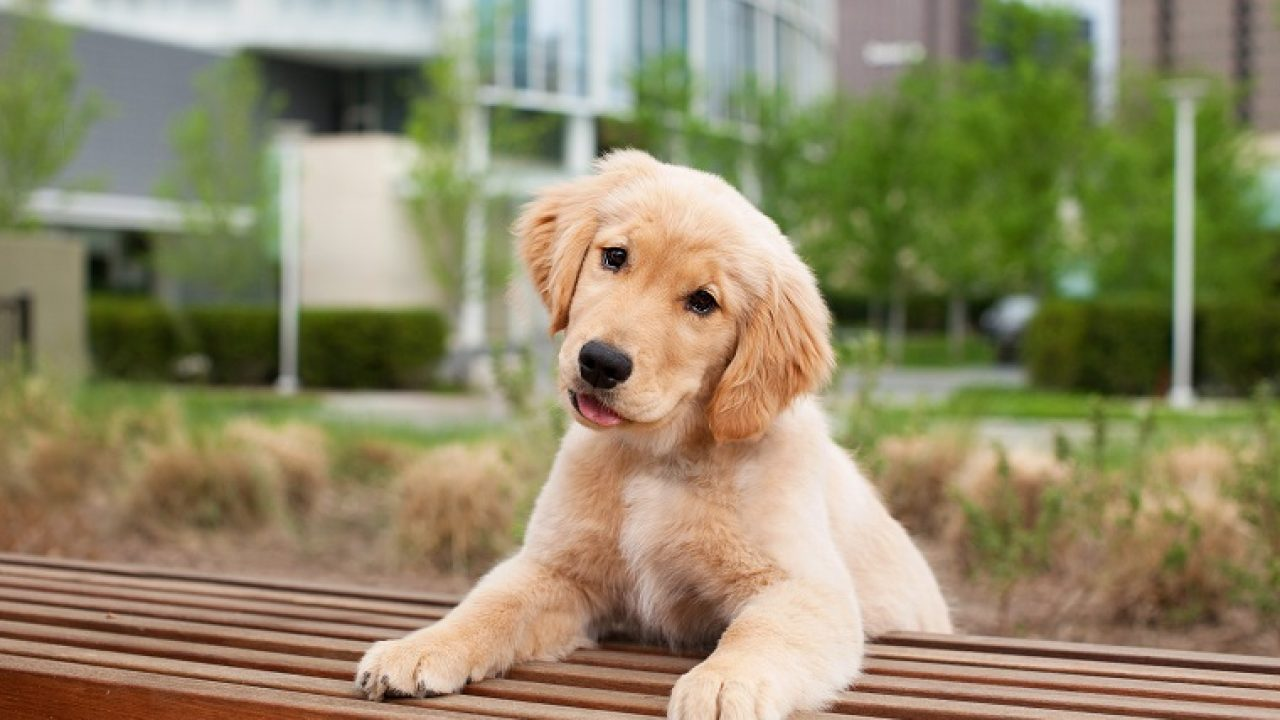
\includegraphics[width = \textwidth]{img/puppies-cover-1280x720}
\end{figure}
\end{Verbatim}

\begin{figure}[H]
\centering % sets horizontal alignment to ``centered''
\caption{A figure}
\label{fig:myfig}
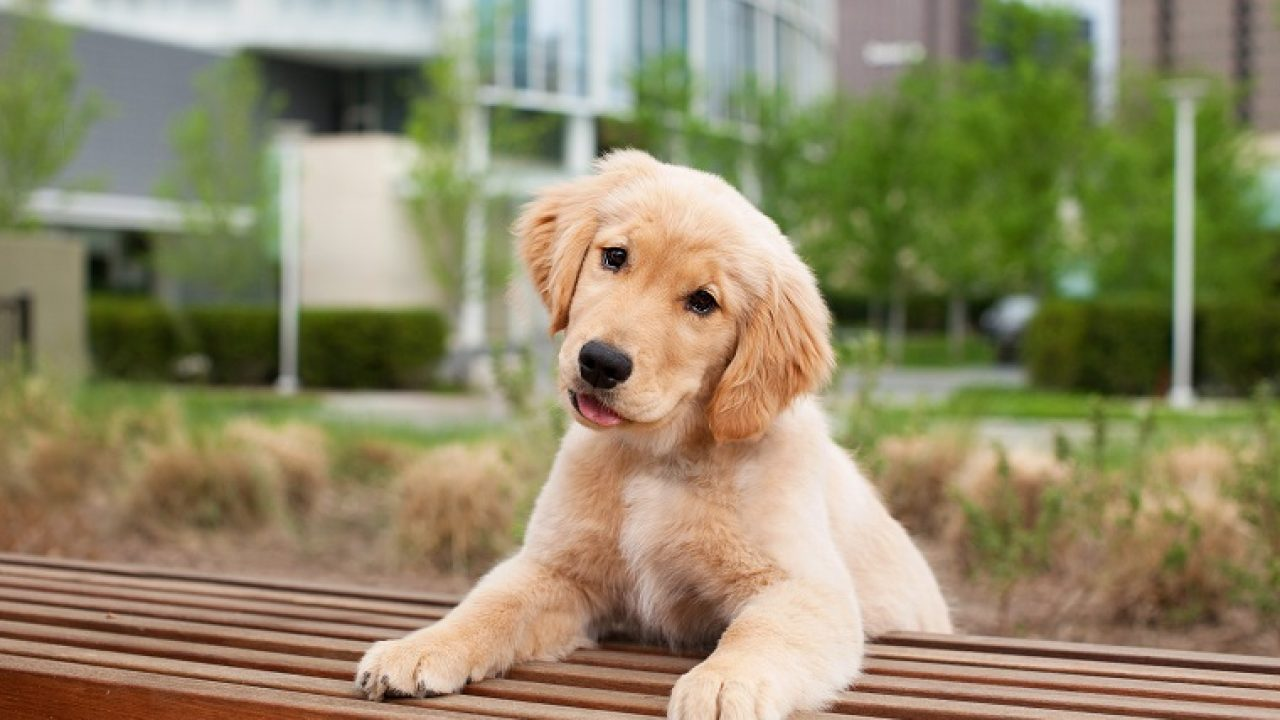
\includegraphics[width = \textwidth]{img/puppies-cover-1280x720}
\end{figure}

Scaling to 0.3 times the text width: 

\begin{Verbatim}[frame=single]
\begin{figure}[H]
\centering % sets horizontal alignment to ``centered''
\caption{A figure, scaled}
\label{fig:myfig}
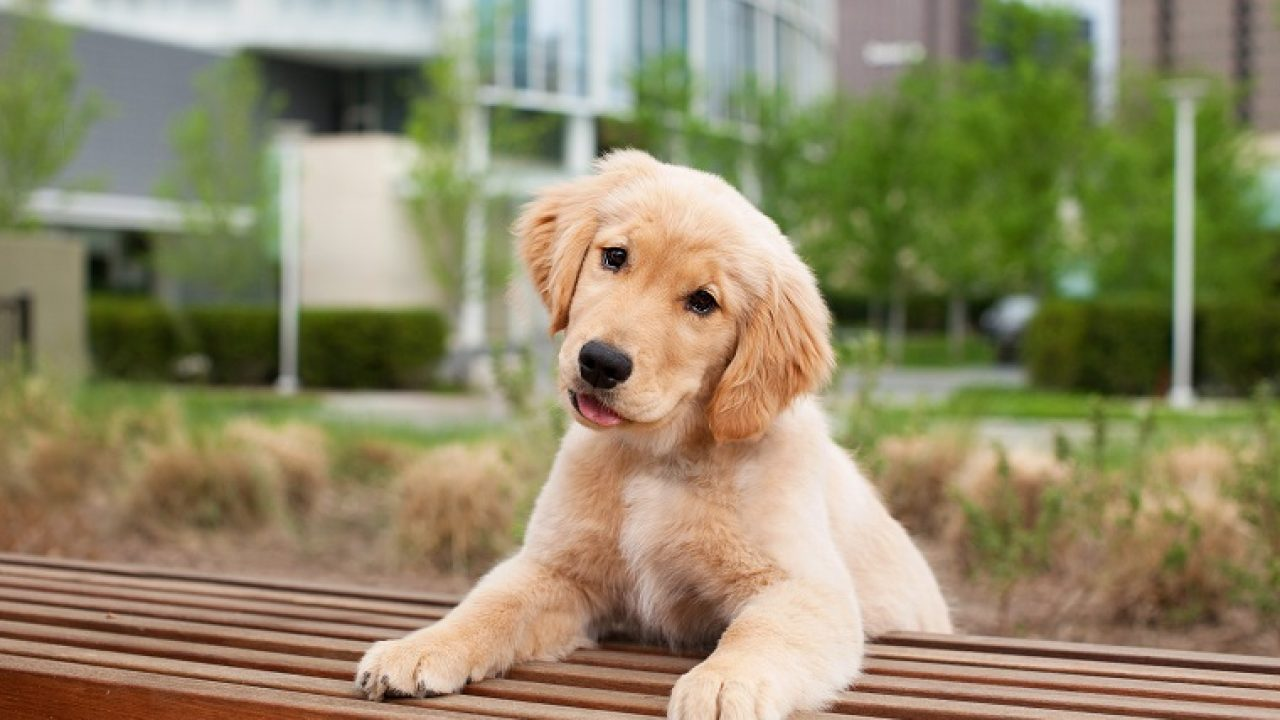
\includegraphics[width = 0.3\textwidth]{img/puppies-cover-1280x720}
\end{figure}
\end{Verbatim}

\begin{figure}[H]
\centering % sets horizontal alignment to ``centered''
\caption{A figure, scaled}
\label{fig:myfig}
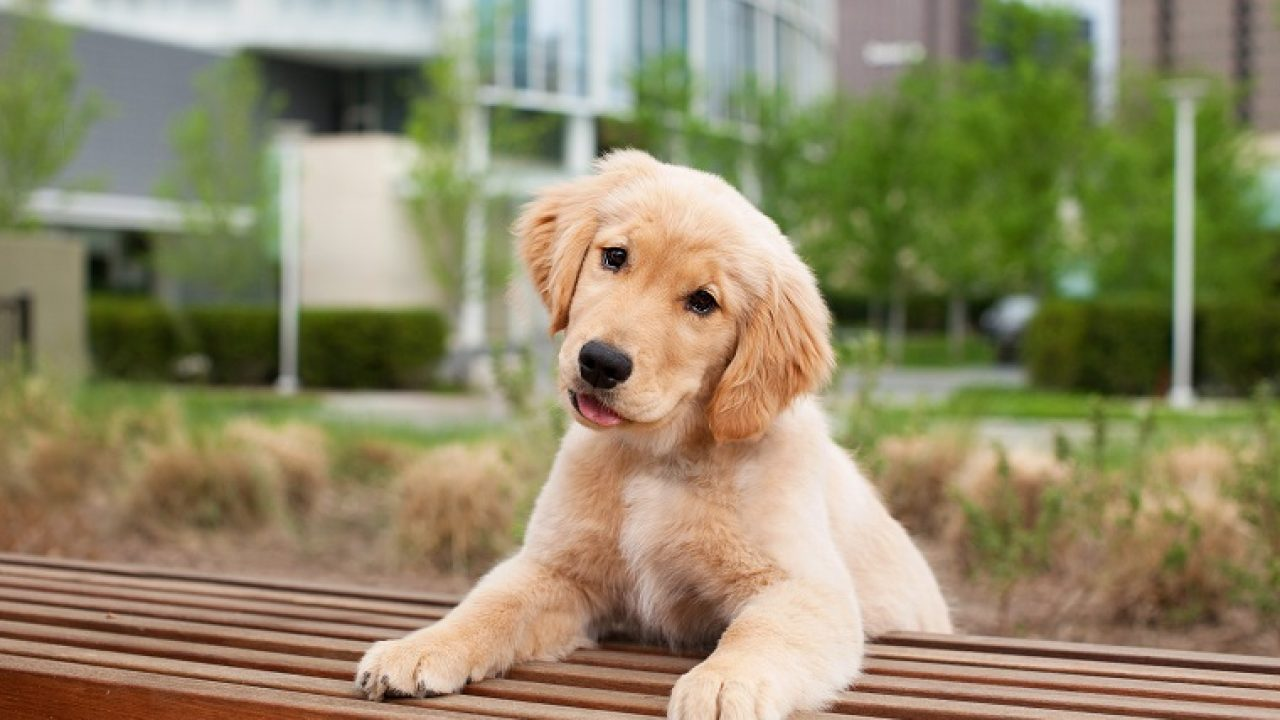
\includegraphics[width = 0.3\textwidth]{img/puppies-cover-1280x720}
\end{figure}

\section{Lists}

Lists in \LaTeX\ can be written without any additional package, but I've found that the \verb#\enumitem# package provides some nice customization (e.g. in changing the formatting of the bullets, symbols, etc.)

To start a \textbf{bulleted} list, use the \verb#itemize# environment and start each new item with the \verb#\item# command:

\begin{Verbatim}[frame=single]
\begin{itemize}
\item Item 1
\item Item 2
\item Item 3
\end{itemize}
\end{Verbatim}

\begin{itemize}
\item Item 1
\item Item 2
\item Item 3
\end{itemize}

To start a \textbf{numbered} list, use the \verb#enumerate# environment, again starting each new item with the \verb#\item# command.

\begin{Verbatim}[frame=single]
\begin{enumerate}
\item Item 1
\item Item 2
\item Item 3
\end{enumerate}
\end{Verbatim}

\begin{enumerate}
\item Item 1
\item Item 2
\item Item 3
\end{enumerate}

To change the style of the list (for instance to use alphabetic letters instead of numbers, make specifications to the ``label'' option of \verb#enumerate#): \footnote{There are many options here, see: https://www.overleaf.com/learn/latex/lists}

\begin{Verbatim}[frame=single]
\begin{enumerate}[label = (\alph*)]
\item Item 1
\item Item 2
\item Item 3
\end{enumerate}
\end{Verbatim}

\begin{enumerate}[label = (\alph*)]
\item Item 1
\item Item 2
\item Item 3
\end{enumerate}


\begin{Verbatim}[frame=single]
\begin{enumerate}[label = (\roman*)]
\item Item 1
\item Item 2
\item Item 3
\end{enumerate}
\end{Verbatim}

\begin{enumerate}[label = (\roman*)]
\item Item 1
\item Item 2
\item Item 3
\end{enumerate}

Last, we can also create nested lists by nesting our enumerate or itemize environments:

\begin{Verbatim}[frame=single]
\begin{enumerate}[label = \alph*.]
\item Item 1
  \begin{itemize}
    \item Nested
  \end{itemize}
\item Item 2
\item Item 3
\end{enumerate}
\end{Verbatim}

\begin{enumerate}[label = \alph*.]
\item Item 1
  \begin{itemize}
    \item Nested
  \end{itemize}
\item Item 2
\item Item 3
\end{enumerate}


\section{Overleaf}

If you aren't doing anything related to \texttt{R}, and just want to typeset text using \LaTeX\ , another neat option is to do all of your writing on \href{https://www.overleaf.com}{Overleaf}, and online platform that allows you to see your changes in real time, collaborate with others in a Google-docs style editing system, and backup your projects automatically using auto-save and version control features. 


\end{document}
